\begin{recipe}
    [% 
        preparationtime = {\unit[40]{min}},
        portion = {\portion{4}},
        bakingtime = {\unit[60]{min}}
    ]
    {Stuffed aubergines}

    \introduction{%
        Another meaty recipe.
        It's quite time-consuming but don't be put off, as the preparation is rather easy.
    }
    \setRecipeLengths{
        ingredientswidth=5.5cm
    }
    \ingredients[13]{%
        2 & Aubergine, big \\
        \unit[500]{g} & Minced beef \\
        \unit[500]{ml} & Passata \\
        1 & Onion \\
        4 & Garlic clove \\
        & Mozzarella \\
        3 hfl. & Olives \\
        \unit[100]{g} & Grated cheddar or Grana Padano  \\
        & Thyme \\
        & Oregano \\
        & Paprika \\
        & Balsamic vinegar
    }

    \preparation{%
        \step Cut aubergines in half.
        Nick across (care not to cut the skin).
        Sprinkle with salt and olive oil, bake at \unit[180]{\textcelcius} for 25-30 min.
        \step Fry onion, at the end add garlic.
        Add mince and fry for 5-7 min.
        \step Core aubergines and chopped flesh add to meat.
        \step Stuff aubergine boats with meat and cover with cheese.
        Beak at  \unit[160-180]{\textcelcius} for about 10 min.
        \vspace{3mm}
        \begin{figure}[h]
            \centering
            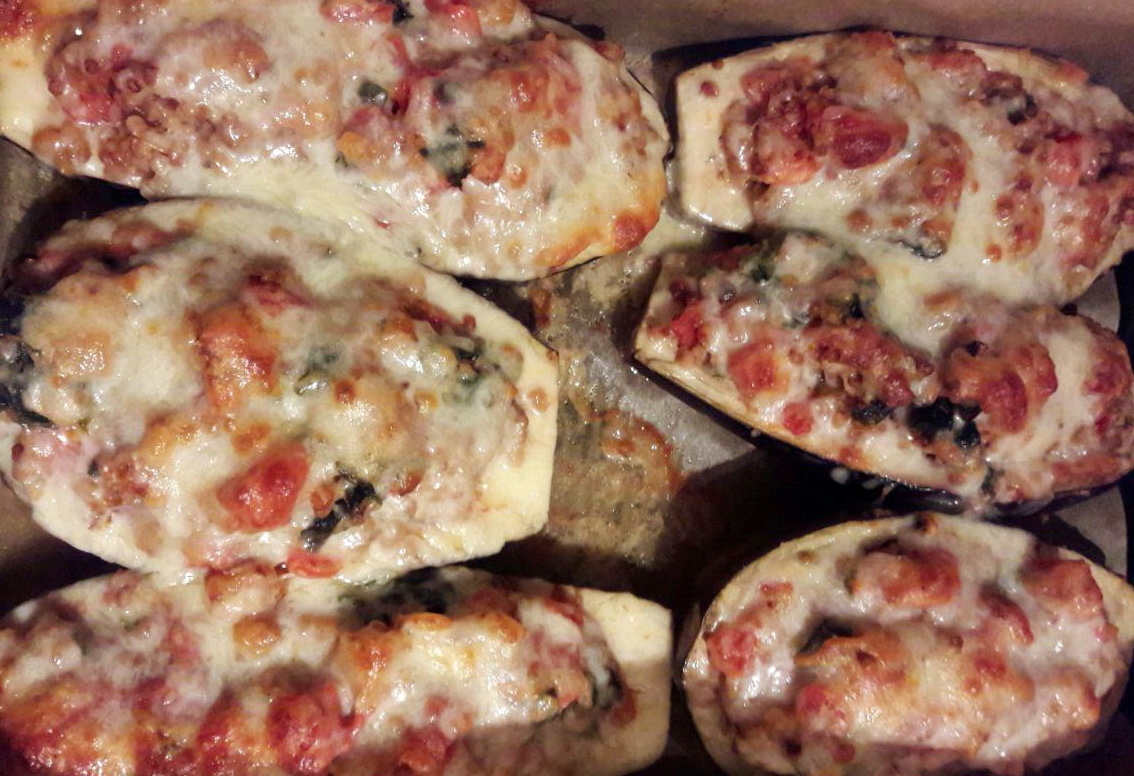
\includegraphics[width=9cm]{pic/stuffed_aubergines}
        \end{figure}
    }

\end{recipe}